 %===================================== CHAP 5 =================================

\chapter{Architecture and implementation}
\label{ch:architecture_and_implementation}

\section{Broker architecture}
\label{sec:architecture_and_implementation-broker_architecture}

This section discusses the high-level aspects of the broker architecture. Some parts of the system are explained in greater detail to provide clear purpose or intent. Additionally, a developer manual can be found in appendix \ref{appendix-developer-manual}.

\subsection{Goals and strategy}
\label{subsec:architecture_and_implementation-broker_architecture-goals_and_strategy}

Building on the results and findings in the research phase, a set of goals were created for the design of the system architecture. Several aspects of the Apollo broker were really well thought trough, and were on the priority list from the start. These included, but were not limited to: Complete protocol agnostic interface. A priority message queue supported by a multi-threaded execution service. Loose coupling of modules, as well as high extendability and low maintenance effort was important and in accordance with the non-functional requirements.

Expanding on these traits, the group wanted a system architecture where each component was a standalone service. A service would expose a public interface from which other components could request data access or services from. Another goal of the design was to have a core service responsible for registering other services, starting them, stopping them, and registering protocols. This would allow the system to be extended by simply registering the new component, without further modifications.

The customer had requested a graphical user interface, and building on experience and knowledge in the group, a web based interface was deemed most appropriate. The group wanted to have an administration interface built using the dynamic properties of the outlined system. Registering a new protocol should not require the administration interface component to be modified. Registering a new core service that a potential developer wanted to expose in the administration interface, should only require adding a new model, Application Programming Interface (herbeby denoted API) controller and template fragment.

Based on these thoughts and ideas, a list of goals were created:

\begin{itemize}
\item The system should not need to know about the details of registered protocols in order to perform as intended. In essence, it should be completely protocol agnostic.
\item Extending the system with new functionality should be as easy as possible.
\item Extending the system with new protocols should be as easy as possible.
\item Extending the system should require as little alteration to existing code as possible.
\item Core functionality should be adhering to the principle of "Separation of concerns" \cite{soc}.
\item Core services should be standalone entities that other components can utilize.
\item The system should have a core service responsible for the entire life cycle of other registered components.
\end{itemize}

\begin{center}
  \begin{figure}[ht!]
    \makebox[\textwidth]{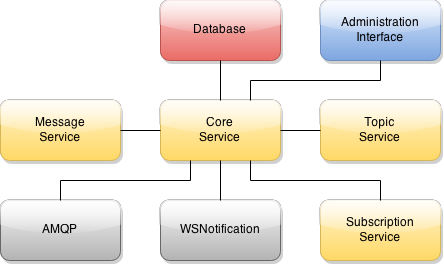
\includegraphics[scale=0.6]{fig/abstract_architecture.png}}
    \caption{High-level system architecture}
    \label{fig:abstract_architecture}
  \end{figure}
\end{center}

With these goals settled, it was apparent that the design outline had properties of a Service Oriented Architecture (hereby denoted SOA) \cite{soa}, as well as the Module Pattern \cite{module-pattern}. This prompted the actual implementation of the system to adhere to these principles and patterns as much as possible, for consistency and future familiarity.

Putting all this together, a high-level system architecture was created (see figure \ref{fig:abstract_architecture}). It illustrates the main entities that were to become the brokering system. Lines between entities illustrate their connection to the core service, which is responsible for all other entity life cycles. Yellow entities are core services in the brokering system, while gray are protocol components.

\subsection{Component dependency}
\label{subsec:architecture_and_implementation-broker_architecture-component_dependency}

The next step was to identify possible critical dependencies and usage dependencies required for a component to provide its complete set of features. This meant that a wide range of scenarios and situations, data flows and potential class structures had to be evaluated. By using the principles of SOA and Module Pattern, the amount of critical dependencies were reduced to a minimum.

Usage dependency could, however, not be reduced to a level lower than what was needed for the system to operate as intended. It was also planned to use event callbacks to handle situations that would have caused extra inter-service dependencies. This would allow services to run regardless of their real-world dependency on other services during certain tasks. An example of this is a situation where a topic is deleted in the administration interface, and subscribers have to be purged from the subscription service. The solution was to have the subscription service listen for topic-related events and update its subscriber set accordingly.

\begin{center}
  \begin{figure}[ht!]
    \makebox[\textwidth]{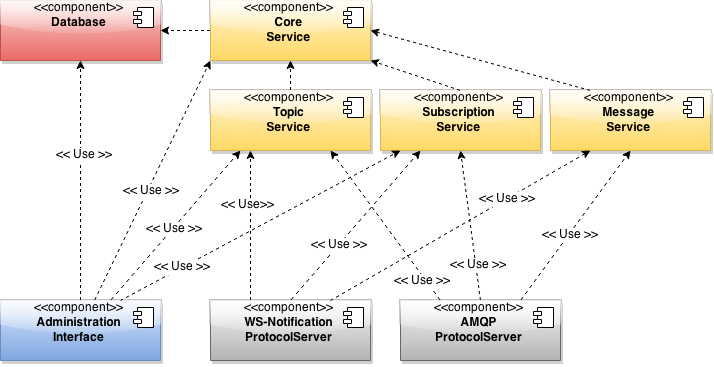
\includegraphics[scale=0.5]{fig/architecture_dependency.png}}
    \caption{Component Dependencies}
    \label{fig:architecture_dependency}
  \end{figure}
\end{center}

After much thought was put into these challenges, a component dependency diagram (see figure \ref{fig:architecture_dependency}) was created to illustrate how the administration interface, services and protocols should depend on each other. As with the high-level architecture, core services are denoted with yellow and protocols with gray.

Dependencies between components that are annotated with $<< Use >>$ represent situations where one component depends on the other to offer its full set of features. In practice, a complete implementation of the brokering system would rely on all these dependencies to meet the specified requirements. But they should not be required for a component to perform its own internal responsibilities. Hence, a single instance of the WSN protocol should be able to run without connectivity to the rest of the system, and fully function in its local environment. This would, however, mean that the rest of the system would be unaware of the subscribers, topics and messages handled by the local instance.

\subsection{Data flow}
\label{subsec:architecture_and_implementation-broker_architecture-data_flow}

\begin{center}
  \begin{figure}[ht!]
    \makebox[\textwidth]{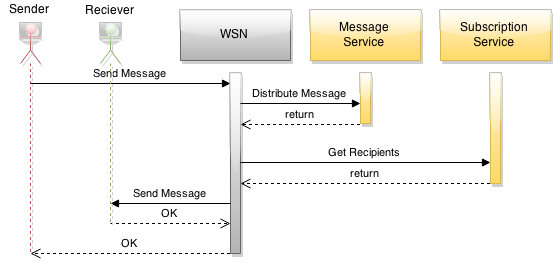
\includegraphics[scale=0.6]{fig/architecture_data_flow_simple.png}}
    \caption{Simplified sequence diagram of possible data flow when sending a notification message using WS-Nu as the protocol library.}
    \label{fig:architecture_data_flow_simple}
  \end{figure}
\end{center}

During the analysis of component dependencies, several potential data flows were analysed. They were used as references when evaluating which components would have critical dependencies and usage dependencies. This proved helpful, as the complexity and scope of what the group had to take into consideration began to dawn at that point. An example of one of these data flows is a possible notification message being sent. A simplified version of the data flow is illustrated in figure \ref{fig:architecture_data_flow_simple}, and assesses requirement FR1.
The figure illustrates which system calls are needed for a sender to send a message, process it, and deliver it. In practice, there might be several receivers and many additional calls, but this has been abstracted away for simplicity.

These simplified sequences were expanded later on, to provide a more realistic data flow in greater detail. During development, the detailed sequences were used as support when implementing proper start up sequences of the different components. Additionally, they were helpful for identifying possible computational bottlenecks, and in providing insight into different ways of structuring the code.

Figure \ref{fig:architecture_data_flow} illustrates an expanded version of what the potential data flow might look like for a send notification message request using WSN. The expanded data flows show occurrences of loops, as well as some of the ideas for inner workings of the components. In this example, the send message call performed in the task runner would invoke a large branch of actions itself. To reduce complexity, the analysis of potential data flows were divided into different segments of the proposed system architecture.

\begin{center}
  \begin{figure}[t]
    \makebox[\textwidth]{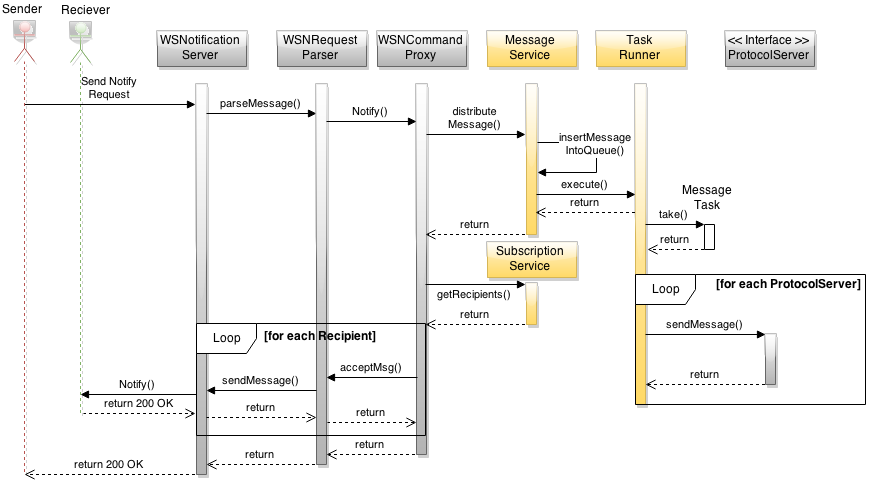
\includegraphics[scale=0.41]{fig/architecture_data_flow.png}}
    \caption{Detailed sequence diagram of possible data flow when sending a notification message using WS-Nu as the protocol library.}
    \label{fig:architecture_data_flow}
  \end{figure}
\end{center}

\section{Broker implementation}
\label{sec:architecture_and_implementation-implementation}

This section provides a brief outline of implementation specific details in the OKSE message brokering system. It lists some common patterns used, choices that were made and the reasoning behind these. The main system components referred to in this section are illustrated in figure \ref{fig:abstract_architecture}. The following sections assume a higher level of technical knowledge, and does not elaborate on every technical term used to describe the implementation. The scope of these terms fall into what can be described as general programming domain knowledge.

\subsection{Core}
\label{subsec:architecture_and_implementation-implementation-core}

As outlined in the architecture design goals, the core components of the system were implemented as standalone services, using the singleton pattern \cite{singleton}. To provide a thread safe execution environment, all services were implemented with an internal task queue. This reactor thread pattern \cite{reactor-pattern} acts as a demultiplexer, collecting requests for service methods from other threads and executing them synchronously by order of arrival.

\subsubsection{CoreService}
\label{subsec:architecture_and_implementation-implementation-core-coreservice}

The CoreService is the main part of the OKSE message translation and brokering system. It is responsible for booting and stopping the registered core services, such as those described in subsequent sections of this chapter. Additionally, the CoreService boots up registered ProtocolServers, which are described in their own section below. The CoreService is also responsible for gracefully shutting down registered ProtocolServers.

As with all the OKSE core services, the main CoreService extends the AbstractCoreService class. This class holds some common attributes that are needed, as well as definitions of the abstract methods for \verb!init()!, \verb!boot()!, \verb!run()! and \verb!stop()! actions. All of these services are intended to follow the singleton pattern, uses static references in the implementation. Thus, the remaining needed methods and fields for initialization and instantiation are not provided by the abstract super class. They have to be implemented using a similar approach as described in the \ref{sec:common-patterns-used} and \ref{sec:adding-new-core-services} chapters. An overview of the boot sequence of the main OKSE components is described in figure \ref{fig:boot-sequence}.


\begin{center}
  \begin{figure}[ht!]
    \makebox[\textwidth]{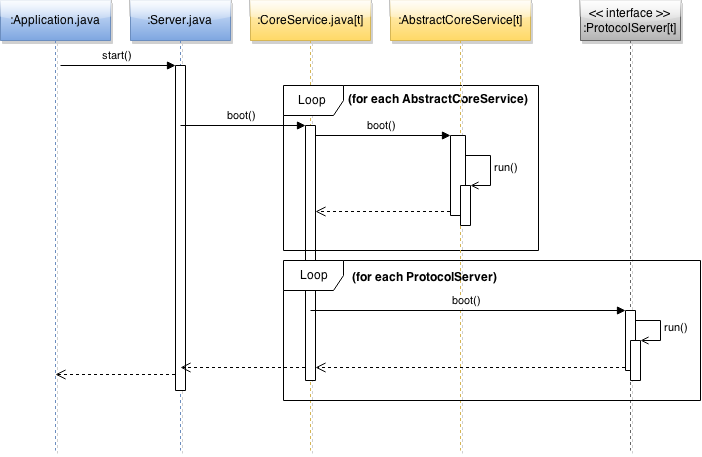
\includegraphics[width=\textwidth]{fig/bootSequence.png}}
    \caption{Boot sequence main components of OKSE}
    \label{fig:boot-sequence}
  \end{figure}
\end{center}

The details of the \verb!init()!, \verb!boot()! and \verb!run()! methods will vary from service to service, and from protocol server to protocol server. After the boot sequence has completed, all of the instances of either core services or protocol servers have their own dedicated thread that awaits the next task or event to execute.

\subsubsection{TopicService}
\label{subsec:architecture_and_implementation-implementation-core-topicservice}

The \verb!TopicService! is responsible for creating, updating and  deleting topics, as well as event propagation for topic related events. It runs as a single threaded reactor that consumes tasks from a blocking queue, securing thread safety. It is also supported by the \verb!TopicTools! class, which provides helper methods for topic tree traversal. It is worth mentioning that all topics that have subpaths will be linked together into a tree, regardless of the fact that none of the implemented protocols use this feature. They were implemented this way to account for future protocols that do support hierarchy based message distribution, and complements the non-functional requirement extendability  (see section \ref{subsec:requirements_engineering-non_functional_requirements-extendibility}) in that way.

The \verb!Topic! object itself has two ways of retrieving its name. A \verb!getName()! which returns the name of that particular node, and a \verb!getFullRawTopicString()! which traverses the tree until a root topic node is found. The latter will return a concatenation of the topic node names found on the path to the root node. A concatenated string of topic names is the default identifier of topics throughout the system.
The \verb!TopicService! implements listener support, which is used by other services that need to know when topics are created or deleted. This is done by implementing \verb!TopicChangeListener! on the respective service's class, and registering it to the \verb!TopicService! using the \verb!addTopicChangeListener()! method.
As topics may be deleted from the administration panel, or new topics could be created through the topic mapping feature, some protocol servers might need to update their local representations. Listener support was used as the preferred way of accomplishing these needs. The reason being that they will be performed as synchronized jobs that secure thread safety.

\subsubsection{SubscriptionService}
\label{subsec:architecture_and_implementation-implementation-core-subscriptionservice}

The \verb!SubscriptionService! is responsible for the creating, updating and deleting subscribers and publishers, as well as event propagation for these types of events. It runs as a single threaded reactor that consumes tasks from a blocking queue, securing thread safety. The \verb!SubscriptionService! implements listener support, which is used by other services that need to know when subscribers or publishers are created, updated or deleted. This is done by implementing \verb!SubscriptionChangeListener! and \verb!Publisher! \verb!ChangeListener! respectively, and registering the class in question to the \verb!SubscriptionService! using the \verb!addSubscriptionChangeListener()! and  \verb!addPublisherChangeListener()! methods. As subscribers and publishers may be deleted from the administration panel, some services or protocol servers may need to update their local representations. Listener support was used as the preferred way of accomplishing these needs.

\subsection{MessageService}
\label{subsec:architecture_and_implementation-implementation-core-messageservice}

The \verb!MessageService! is responsible for distribution of messages, as well as duplicating messages if topic mappings are present. The \verb!MessageService! delegates much of the actual work to the \verb!CoreService!'s thread pool, which in turn schedules the messages to be sent. It runs as a single threaded reactor that consumes message distribution requests from a blocking queue, securing thread safety.
When a message is received for distribution, it is added into the \verb!MessageService!'s message queue, and consumed in order of arrival. In turn, the \verb!MessageService! iterates through all registered protocol servers, and calls the \verb!sendMessage()! method on each. Each of these calls are executed as a runnable job which is dispatched to the \verb!CoreService!'s central thread pool.

It is important to note that the \verb!MessageService! is oblivious to how protocol servers handle messages locally. This means that the \verb!MessageService! will call the \verb!send! \verb!Message()! method on the same protocol server as the message was received from. This allows the protocol server implementations to choose how they handle message distribution. A requirement is that they check the \verb!originProtocol! field of the message in their \verb!send!\verb!Message()! method, to prevent messages from entering an infinite loop.

Additionally, the \verb!MessageService! keeps the latest messages sent on a topic in local cache, so that protocols like WSN that require this feature can retrieve them. In order to update the local latest message cache, the \verb!MessageService! is registered as a listener to \verb!TopicChangeEvent!s, to respond appropriately if topics are deleted from the administration panel.

\subsubsection{ProtocolServer}
\label{subsec:architecture_and_implementation-implementation-core-protocolserver}

The \verb!ProtocolServer! interface contains the common methods required in the general life cycle of a \verb!ProtocolServer!. This interface is implemented in the \verb!Abstract! \verb!ProtocolServer! class, which in turn provides some template functionality that is common to all protocol servers.

\subsection{WSN}
\label{subsec:architecture_and_implementation-implementation-wsn}

\begin{center}
  \begin{figure}[ht!]
    \makebox[\textwidth]{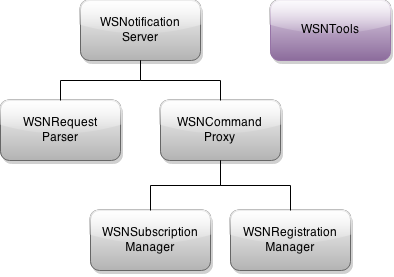
\includegraphics[width=0.6\textwidth]{fig/WSNotificationServer.png}}
    \caption{Component layout for WSN implementation}
    \label{fig:wsnotification-server-structure}
  \end{figure}
\end{center}

WS-Nu was chosen as the implementation library for the WSN protocol.
In order to intercept messages and actions in the WS-Nu library, several of the main WS-Nu components had to be overridden and reimplemented. This led to a structure of components described in figure \ref{fig:wsnotification-server-structure}. The main constituents of the OKSE WSN implementation are the \verb!WSNotification! \verb!Server!, which runs the actual web server sending and receiving requests. The \verb!WSN! \verb!RequestParser!, which is responsible for parsing incoming messages and invoking corresponding methods on the appropriate component. The \verb!WSN!\verb!CommandProxy!, which implements most of the methods defined in the WSN standards document. The command proxy is the parent component of the \verb!WSNSubscription! \verb!Manager! and \verb!WSNRegistrationManager!. The two latter components are responsible for the local state and mapping between subscriber objects and publisher objects respectively.

It is important to note that there are shortcomings in the implementation of the WSN protocol. Some are based on fundamental challenges related to message translation to and from XML-based protocols, and others are errors in the WS-Nu library. These shortcomings are not listed in this chapter, but are described in detail in chapter \ref{subsec:evaluation-implementation-wsn}.

\subsubsection{WSNotificationServer}
At the base of the WSN implementation lies the \verb!WSNotificationServer! class. Like the core services, the server runs as a singleton. The component is responsible for managing an instance of the Jetty Web server, which is connected to a \verb!Handler! class that processes incoming requests. The component also handles outgoing connections using a Jetty Web Client instance. When a request is received, it is processed through the \verb!Handler!. If no errors have occurred during initial handling, it is passed on to the \verb!WSNRequestParser!. Based on the results from the request parser call, an appropriate response message is generated and returned to the requesting client.

In the event of an outgoing message being sent, the \verb!sendMessage()! method of the \verb!WSNotification!\verb!Server! is invoked, and a connection is made by the Jetty Client instance to the subscribers destination address. Depending on whether the message originated from WSN or was translated from another protocol, additional steps are included. In the latter case, a WS-Nu message object is first created containing the relevant information, before dispatching it to the \verb!WSNRequest!\verb!Parser! like any other WSN message.

\subsubsection{WSNRequestParser}
The \verb!WSNRequestParser! is the OKSE implementation of what is considered a \verb!Hub! in WS-Nu. All WSN requests to the OKSE message broker will pass through the request parser. The main tasks of the \verb!WSNRequestParser! is to analyze requests and deliver them to the appropriate services, to generate valid outgoing message structures, and to accept WS-Nu internal messages for distribution. 

It also acts as a service registry, which holds the \verb!WSNCommandProxy!, \verb!WSNSubscri! \verb!ptionManager! and \verb!WSNRegistration! \verb!Manager! as potential recipient services. When accepting an internal message, the request parser will attempt to identify which of the registered services that are eligible to process the request message. If none are eligible, a standard "not found" response message is delivered to the \verb!WSNotification!\verb!Server! and relayed back to the requesting client.

\subsubsection{WSNCommandProxy}

The \verb!WSNCommandProxy! is the main WSN brokering implementation. It contains most of the required methods defined in the WSNotification standard, and exposes methods for processing these different types of actions. It is implemented as a web service that is registered to the \verb!WSNRequestParser!, and accepts requests for the service methods it exposes. Since the command proxy is an extension of the WS-Nu abstract notification broker class, it interacts seamlessly with the rest of the WS-Nu components. The command proxy also holds an instance of the \verb!WSNSubscriptionManager! and \verb!WSNRegistrationManager! classes, and delegates some of its responsibilities to these instances. This module assesses most of the requirements related to the structure of WSN, specifically FR1 to FR6 and FR10 (see section \ref{sec:requirements_engineering-functional_requirements}).

\subsubsection{WSNSubscriptionManager}

The \verb!WSNSubscriptionManager! is responsible for keeping track of the local subscriber representations in WS-Nu and their relations to the OKSE subscriber representation. It is implemented as a web service that is registered to the \verb!WSNRequestParser!, and accepts requests for the service methods it exposes. Since the subscription manager is an extension of the WS-Nu abstract subscription manager, it interacts seamlessly with the rest of the WS-Nu components.

As an example, requests to subscribe or unsubscribe is relayed through the \verb!WSNSubs! \verb!criptionManager!, which in turn calls the OKSE \verb!Subscription!\verb!Service!. Since this is merely an intermediate manager to translate from WS-Nu to OKSE behaviour, the \verb!WSNSubscriptionManager! is registered as a listener to the OKSE \verb!Subscription! \verb!Service!. In the event of a new subscriber, the local WS-Nu subscription representation is stored in the manager, and an \verb!addSubscriber()! call is made to the OKSE \verb!SubscriptionService!.

In the event of an unsubscribe request, a \verb!removeSubscriber()! call is performed directly to the OKSE \verb!SubscriptionService!. The manager then awaits a callback through its listener support, as a confirmation that it is okay to finally remove the local WS-Nu subscription representation.
This kind of control flow allows the manager to automatically update itself. 
In the event of a subscriber being forcefully removed from the administration interface, or its subscription having expired in the OKSE \verb!SubscriptionServi! \verb!ce!, the manager will be updated through this event callback mechanism.
The subscription manager assesses the functional requirements related to the subscribe mechanisms of WSN. Specifically FR7, 8 and 9 (see section \ref{sec:requirements_engineering-functional_requirements}).

\subsubsection{WSNRegistrationManager}

The \verb!WSNRegistrationManager! is responsible for keeping track of the local publisher representations in WS-Nu and their relations to the OKSE publisher representation. It is implemented as a web service that is registered to the \verb!WSNRequestParser!, and accepts requests for the service methods it exposes. Since the registration manager is an extension of the WS-Nu abstract publisher/registration manager, it interacts seamlessly with the rest of the WS-Nu components.

Similar to the \verb!WSNSubscriptionManager!, the \verb!WSNRegistrationManager! handles a local representation of registered publishers. It creates a local entry when a register-publisher request arrives, and delegates unregister requests directly to the OKSE \verb!SubscriptionService!. This, in turn, allows the \verb!WSNRegistrationManager! to automatically update itself based on the events it listens to, in the same manner as the \verb!WSNSubscriptionManager!.

\subsection{AMQP}
\label{subsec:architecture_and_implementation-implementation-amqp}
The implementation of AMQP mainly consists of two parts. The first part is the handling of AMQP decoding and encoding of messages and the handling of the AMQP data in the network requests and responses. The second part is the handling of broker behaviour and the integration with the rest of the system. 

As every protocol server is implemented to run on a single thread, there is a need to handle the incoming and outgoing requests/messages in an efficient way. After some consideration, the AMQP protocol server was implemented using the reactor event loop pattern \cite{event-loop}. 
The AMQP network socket was implemented using the Java non-blocking I/O library. The benefits of using a non-blocking socket is that instead of having to devote one thread per client, it will instead keep multiple channels open and perform multiplexing. This is ideal for the single thread approach, as no single client will halt the program when it has stopped sending data. After the input is received and has been demultiplexed, Qpid (see section \ref{subsub-apache_qpid_proton}) will convert the incoming data to an event, which is then added to the event queue.

Simultaneously with the event queue getting new events, the event loop is continuously dispatching the events to the correct methods on different handlers. A handler is a class that extends the \verb!BaseHandler! class from Qpid. The handler can override event methods invoked by the event queue. The AMQP implementation has the following handlers; \verb!AMQPServer!, \verb!Driver!, \verb!Handshaker! and \verb!SubscriptionHandler!, with their own specific task.

\begin{center}
  \begin{figure}[ht!]
    \makebox[\textwidth]{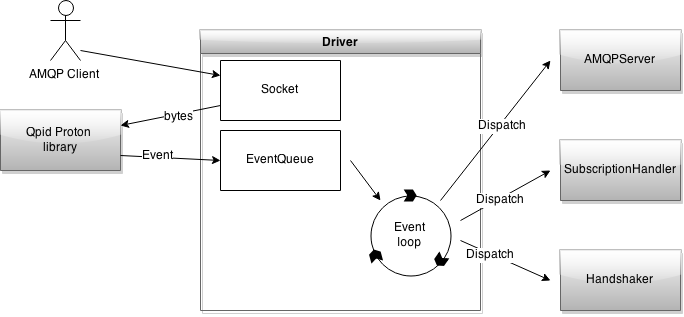
\includegraphics[width=\textwidth]{fig/amqp_recv.png}}
    \caption{AMQP Receive implementation overview}
    \label{fig:amqp_recv}
  \end{figure}
\end{center}

\subsubsection{AMQPServer}
The AMQPServer handler is responsible for the incoming and outgoing messages. It handles the messages that come from AMQP producers and the internal messages from other protocols. It has an internal message queue where messages are stored until the corresponding event is triggered. It handles conversion of messages from AMQP format to the OKSE internal representation, and dispatching to the message service. It is implemented with optimizations to get AMQP messages out fast, and to prevent loops. When an AMQP message is received, it will automatically dispatch the AMQP message back to AMQP subscribers, and the OKSE message to the WSN subscribers. Figure \ref{fig:amqp_recv} and \ref{fig:amqp_send} shows an architectural overview of AMQPServer.

\subsubsection{Driver}
The event loop and the socket logic is implemented in the Driver class. This class is responsible for accepting incoming connections, and handle the incoming requests. After a connection is opened with a client, every request received is passed to Qpid, which decodes the instruction and adds it back to the Driver in the form of an event. The event is added straight to a collector, which is used as the event queue. The event loop that is running continuously, will dispatch events as long as there are any in the queue. If there are no events, it will enter a wait state. The driver is responsible for the handling of requirement FR11 (see section \ref{sec:requirements_engineering-functional_requirements}).

\subsubsection{SubscriptionHandler}
In the \verb!SubscriptionHandler! class, subscribers and their routes/topics are processed. Additionally, it handles the basic information about a sender/producer and the integration with the OKSE SubscriptionService. The functionality in this handler is based on addition and removal of subscribers. When a subscribe request occurs, the handler will add the user to the internal subscriber map, before adding the subscriber to the OKSE SubscriptionService. When a subscriber disconnects, it removes the disconnected subscriber in the same manner. This class assesses the the requirements FR12 and FR13 (see section \ref{sec:requirements_engineering-functional_requirements}), about subscribing using AMQP.

\subsubsection{Handshaker}
The Handshaker handles all of the open and close events of a connection. It makes sure that the initiation of the connection, session and link is done properly. It also ensures that it is closed properly when the link is broken or disconnected.

\begin{center}
  \begin{figure}[ht!]
    \makebox[\textwidth]{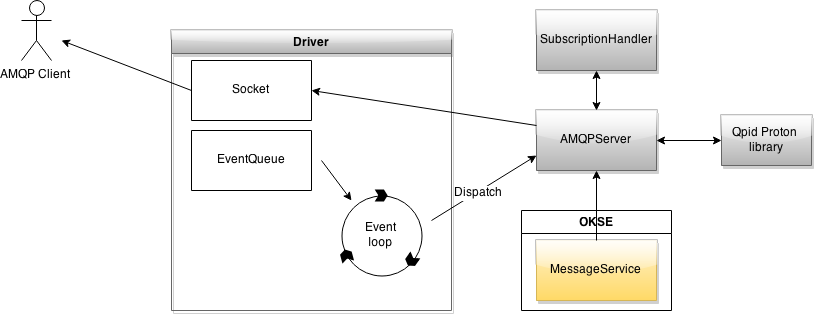
\includegraphics[width=\textwidth]{fig/amqp_send.png}}
    \caption{AMQP Send implementation overview}
    \label{fig:amqp_send}
  \end{figure}
\end{center}

\subsubsection{Queue vs Topic behavior}
WSN and AMQP use different behaviour for handling topics/queues. As WSN is a pure publish/subscribe protocol, it is only concerned with topics. A description of the difference between topics and queues can be found in chapter \ref{subsec:architecture_and_implementation-topic_and_queue_differecnce}.

In the initial implementation, the system only complied with the given standards for each protocol. To cope with the differences, the group implemented logic to handle the conversion between the two behaviours. In addition, the group consulted the customer with the idea of implementing a non-standard topic implementation of AMQP. This meant that AMQP could be used with the same behaviour as WSN, and that all AMQP subscribers on one topic/queue would receive the message. The customer liked the idea, as it would fit nicely with their usage pattern. 

A configuration switch was implemented to select which mode to use. The switch is available through the configuration file and the administration interface. The logic for this feature is implemented in AMQPServer which, as previously stated, is responsible for the outgoing message logic.


\section{User interface}
\label{sec:architecture_and_implementation-user_interface}

One of the initial requirements from the customer, was to have a graphical user interface. This was supposed to display relevant data and allow the administrator to moderate topics and subscriptions. After an initial consideration, the Spring Framework was chosen to be the most suitable framework (see section  \ref{subsec:prestudies-tools-spring_mvc}) for building the administration panel. The user interface was implemented using the MVC-pattern. 

\subsection{Design}
\label{subsec:architecture_and_implementation-user_interface-design}

As previously stated, a considerable amount of time was spent researching the Apollo broker during the research phase. This provided information about what an administration interface should provide. The customer had initially not stated any specific requirements for the administration panel. Therefore, an initial administration user interface wireframe was created and shown to the customer. The wireframe was heavily influenced by Apollo. This wireframe (see figure \ref{fig:initial_prototype}), along with the creation of use cases, set the terms for creating a prototype.

The group agreed upon creating a functional prototype for the customer. This prototype was made available, so that the customer could provide feedback. During most customer meetings, the current version of the administration interface was discussed. The customer gave feedback on how new elements in the panel met the customers expectations. This approach gave the group great advantage; rapid response from the customer, which made it easy to improve the interface and add additional features. Throughout the lifetime of the development phase, the administration panel was continuously deployed on the test server.

\begin{center}
  \begin{figure}[ht!]
    \makebox[\textwidth]{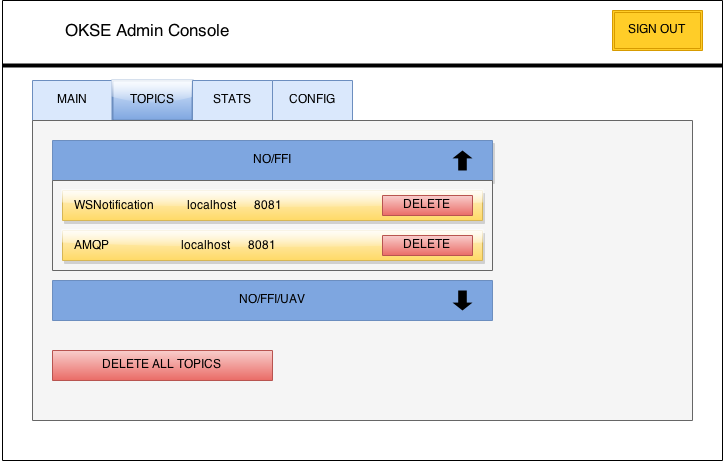
\includegraphics[scale=0.5]{fig/initial_prototype.png}}
    \caption{Initial website wireframe}
    \label{fig:initial_prototype}
  \end{figure}
\end{center}

The final interface contains six panes; "Main", "Topics", "Subscribers", "Statistics", "Logs" and "Configuration". The "Main"-pane contains information about the message broker. It is meant to give a general overview of the current operating environment, as well as the system status and memory usage. The "Statistics"-pane contains useful statistics about requests, messages etc on the different protocols. The "Logs"-pane contains runtime logs for debugging purposes. The "Topics"-pane shows all registered topics in the message broker and information about the current topics, as well as the possibility to remove them. The "Subscribers"-pane has the same functionality as the "Topics"-pane, but for subscribers. Finally, in the "Configuration"-pane, the user can change the brokers settings and map topics together. Also, a possibility to add relays between multiple OKSE brokers is located here. A user manual, including a visual guide to the interface, can be found in appendix \ref{appendix-user-manual}.

\subsection{Implementation}
\label{subsec:architecture_and_implementation-implementation}

The OKSE administration interface was designed in a modularized way, to achieve loose coupling as defined by the modularization requirement (see section  \ref{subsec:requirements_engineering-non_functional_requirements-modularization}). Each pane of the interface would have its own controller and a respective front-end JavaScript file. The advantage of this approach was having the administration panel designed as a single page web application. The page uses AJAX-requests to reach a representational state transfer (hereby denoted REST) API. By using the Spring Framework, the system exposes API-endpoints which can be used to access and/or modify data. This is the main data source for the front-end and is a critical part of the single page design. Translated to the MVC-pattern, the Spring Framework work as a controller through REST-controllers, and the different panes work as views. Each AJAX-request to the API-endpoints will reach the controllers and modify the models and/or message broker. Structuring the system this way gives some advantages: 

\begin{itemize}
    \item No need to refresh the entire administration panel.
    \item One controller class serves one pane; easy to debug.
    \item Loose coupling, no dependencies between panes.
    \item Easy to extend the application further.
\end{itemize}

\begin{center}
  \begin{figure}[ht!]
    \makebox[\textwidth]{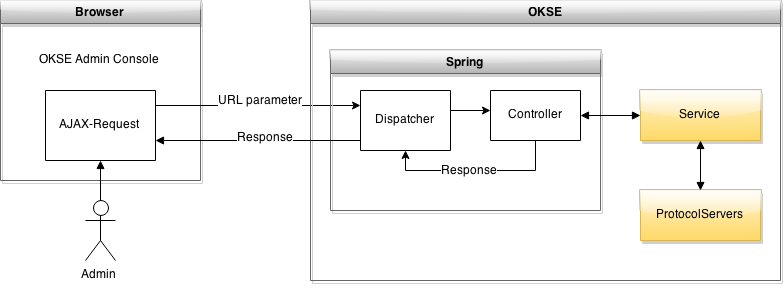
\includegraphics[width=\textwidth]{fig/oacRequestFlow.png}}
    \caption{Request flow for the administration interface}
    \label{fig:oac-request-flow}
  \end{figure}
\end{center}

\subsubsection{Back-end}

The back-end of OKSE works as a RESTful Web Service. It works as a link between the administration interface and all different registered services in OKSE. Figure \ref{fig:oac-request-flow} shows an overview of how a request is handled by the server. The key concepts to notice here are the AJAX-requests and the controllers. On an event, whether it is a page auto update or a button-click, the request URL is accessed by an AJAX-request. Springs dispatcher maps the URL and forwards it to the correct controller. This controller interacts with OKSE's services and returns a response. 

\subsubsection{Front-end}

The front-end of OKSE is the only component of the system that is directly accessible for graphical user interaction. It is responsible for making HTTP-requests to the back-end for manipulation and presentation of the state that the system is currently in. To ensure and minimize the probability for cross-browser incompatibilities, the front-end is implemented using the jQuery framework. Each pane of the administration interface has its own module implemented with jQuery. These modules are responsible for event-handling, AJAX-requests and updating of information in their respective pane.
For a more detailed description about the administration interface architecture, see appendix \ref{appendix-developer-manual}.

\clearpage
